\documentclass[1p]{elsarticle_modified}
%\bibliographystyle{elsarticle-num}

%\usepackage[colorlinks]{hyperref}
%\usepackage{abbrmath_seonhwa} %\Abb, \Ascr, \Acal ,\Abf, \Afrak
\usepackage{amsfonts}
\usepackage{amssymb}
\usepackage{amsmath}
\usepackage{amsthm}
\usepackage{scalefnt}
\usepackage{amsbsy}
\usepackage{kotex}
\usepackage{caption}
\usepackage{subfig}
\usepackage{color}
\usepackage{graphicx}
\usepackage{xcolor} %% white, black, red, green, blue, cyan, magenta, yellow
\usepackage{float}
\usepackage{setspace}
\usepackage{hyperref}

\usepackage{tikz}
\usetikzlibrary{arrows}

\usepackage{multirow}
\usepackage{array} % fixed length table
\usepackage{hhline}

%%%%%%%%%%%%%%%%%%%%%
\makeatletter
\renewcommand*\env@matrix[1][\arraystretch]{%
	\edef\arraystretch{#1}%
	\hskip -\arraycolsep
	\let\@ifnextchar\new@ifnextchar
	\array{*\c@MaxMatrixCols c}}
\makeatother %https://tex.stackexchange.com/questions/14071/how-can-i-increase-the-line-spacing-in-a-matrix
%%%%%%%%%%%%%%%

\usepackage[normalem]{ulem}

\newcommand{\msout}[1]{\ifmmode\text{\sout{\ensuremath{#1}}}\else\sout{#1}\fi}
%SOURCE: \msout is \stkout macro in https://tex.stackexchange.com/questions/20609/strikeout-in-math-mode

\newcommand{\cancel}[1]{
	\ifmmode
	{\color{red}\msout{#1}}
	\else
	{\color{red}\sout{#1}}
	\fi
}

\newcommand{\add}[1]{
	{\color{blue}\uwave{#1}}
}

\newcommand{\replace}[2]{
	\ifmmode
	{\color{red}\msout{#1}}{\color{blue}\uwave{#2}}
	\else
	{\color{red}\sout{#1}}{\color{blue}\uwave{#2}}
	\fi
}

\newcommand{\Sol}{\mathcal{S}} %segment
\newcommand{\D}{D} %diagram
\newcommand{\A}{\mathcal{A}} %arc


%%%%%%%%%%%%%%%%%%%%%%%%%%%%%5 test

\def\sl{\operatorname{\textup{SL}}(2,\Cbb)}
\def\psl{\operatorname{\textup{PSL}}(2,\Cbb)}
\def\quan{\mkern 1mu \triangleright \mkern 1mu}

\theoremstyle{definition}
\newtheorem{thm}{Theorem}[section]
\newtheorem{prop}[thm]{Proposition}
\newtheorem{lem}[thm]{Lemma}
\newtheorem{ques}[thm]{Question}
\newtheorem{cor}[thm]{Corollary}
\newtheorem{defn}[thm]{Definition}
\newtheorem{exam}[thm]{Example}
\newtheorem{rmk}[thm]{Remark}
\newtheorem{alg}[thm]{Algorithm}

\newcommand{\I}{\sqrt{-1}}
\begin{document}

%\begin{frontmatter}
%
%\title{Boundary parabolic representations of knots up to 8 crossings}
%
%%% Group authors per affiliation:
%\author{Yunhi Cho} 
%\address{Department of Mathematics, University of Seoul, Seoul, Korea}
%\ead{yhcho@uos.ac.kr}
%
%
%\author{Seonhwa Kim} %\fnref{s_kim}}
%\address{Center for Geometry and Physics, Institute for Basic Science, Pohang, 37673, Korea}
%\ead{ryeona17@ibs.re.kr}
%
%\author{Hyuk Kim}
%\address{Department of Mathematical Sciences, Seoul National University, Seoul 08826, Korea}
%\ead{hyukkim@snu.ac.kr}
%
%\author{Seokbeom Yoon}
%\address{Department of Mathematical Sciences, Seoul National University, Seoul, 08826,  Korea}
%\ead{sbyoon15@snu.ac.kr}
%
%\begin{abstract}
%We find all boundary parabolic representation of knots up to 8 crossings.
%
%\end{abstract}
%\begin{keyword}
%    \MSC[2010] 57M25 
%\end{keyword}
%
%\end{frontmatter}

%\linenumbers
%\tableofcontents
%
\newcommand\colored[1]{\textcolor{white}{\rule[-0.35ex]{0.8em}{1.4ex}}\kern-0.8em\color{red} #1}%
%\newcommand\colored[1]{\textcolor{white}{ #1}\kern-2.17ex	\textcolor{white}{ #1}\kern-1.81ex	\textcolor{white}{ #1}\kern-2.15ex\color{red}#1	}

{\Large $\underline{12n_{0292}~(K12n_{0292})}$}

\setlength{\tabcolsep}{10pt}
\renewcommand{\arraystretch}{1.6}
\vspace{1cm}\begin{tabular}{m{100pt}>{\centering\arraybackslash}m{274pt}}
\multirow{5}{120pt}{
	\centering
	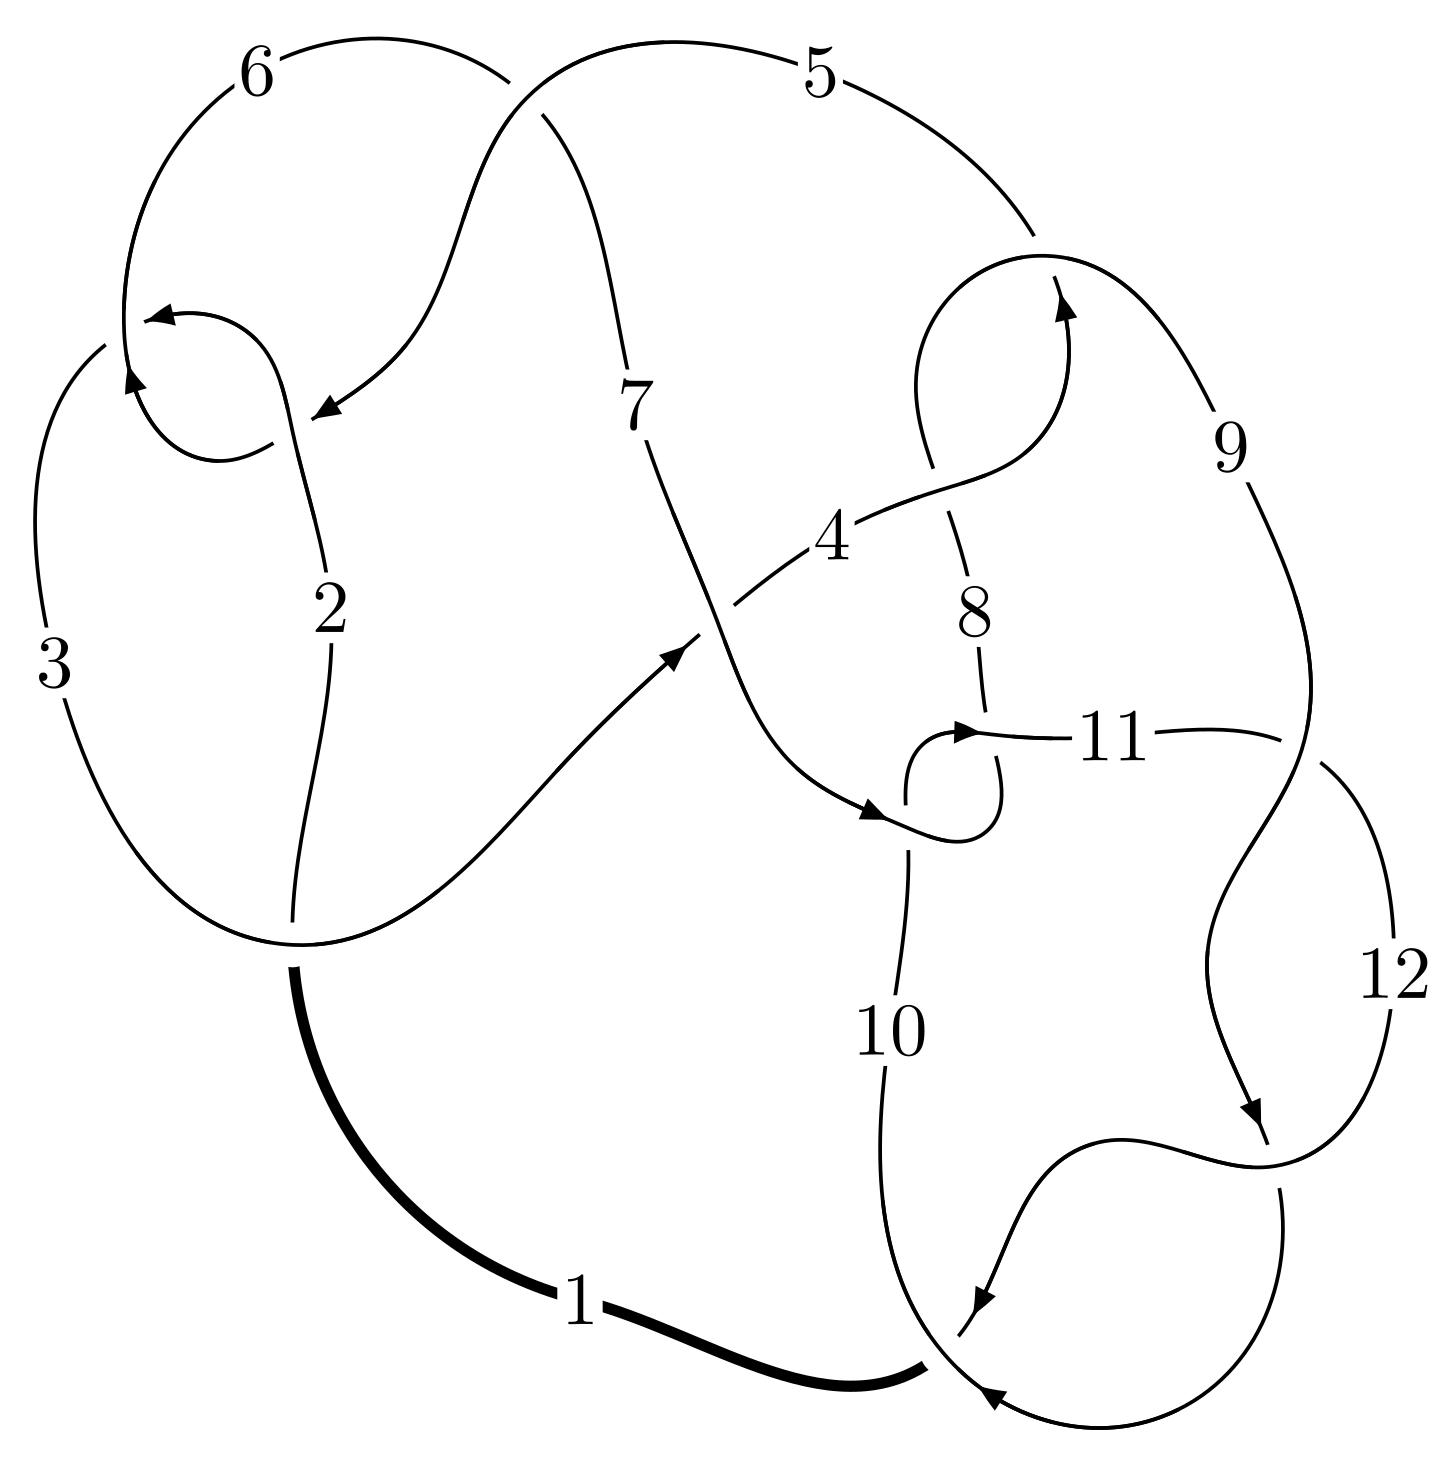
\includegraphics[width=112pt]{../../../GIT/diagram.site/Diagrams/png/2381_12n_0292.png}\\
\ \ \ A knot diagram\footnotemark}&
\allowdisplaybreaks
\textbf{Linearized knot diagam} \\
\cline{2-2}
 &
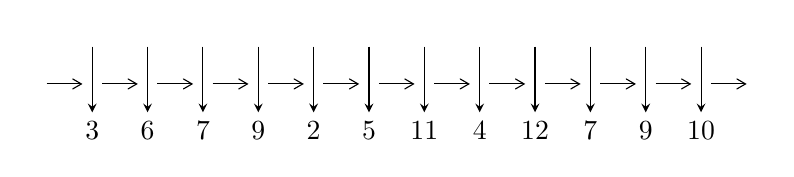
\begin{tikzpicture}[x=20pt, y=17pt]
	% nodes
	\node (C0) at (0, 0) {};
	\node (C1) at (1, 0) {};
	\node (C1U) at (1, +1) {};
	\node (C1D) at (1, -1) {3};

	\node (C2) at (2, 0) {};
	\node (C2U) at (2, +1) {};
	\node (C2D) at (2, -1) {6};

	\node (C3) at (3, 0) {};
	\node (C3U) at (3, +1) {};
	\node (C3D) at (3, -1) {7};

	\node (C4) at (4, 0) {};
	\node (C4U) at (4, +1) {};
	\node (C4D) at (4, -1) {9};

	\node (C5) at (5, 0) {};
	\node (C5U) at (5, +1) {};
	\node (C5D) at (5, -1) {2};

	\node (C6) at (6, 0) {};
	\node (C6U) at (6, +1) {};
	\node (C6D) at (6, -1) {5};

	\node (C7) at (7, 0) {};
	\node (C7U) at (7, +1) {};
	\node (C7D) at (7, -1) {11};

	\node (C8) at (8, 0) {};
	\node (C8U) at (8, +1) {};
	\node (C8D) at (8, -1) {4};

	\node (C9) at (9, 0) {};
	\node (C9U) at (9, +1) {};
	\node (C9D) at (9, -1) {12};

	\node (C10) at (10, 0) {};
	\node (C10U) at (10, +1) {};
	\node (C10D) at (10, -1) {7};

	\node (C11) at (11, 0) {};
	\node (C11U) at (11, +1) {};
	\node (C11D) at (11, -1) {9};

	\node (C12) at (12, 0) {};
	\node (C12U) at (12, +1) {};
	\node (C12D) at (12, -1) {10};
	\node (C13) at (13, 0) {};

	% arrows
	\draw[->,>={angle 60}]
	(C0) edge (C1) (C1) edge (C2) (C2) edge (C3) (C3) edge (C4) (C4) edge (C5) (C5) edge (C6) (C6) edge (C7) (C7) edge (C8) (C8) edge (C9) (C9) edge (C10) (C10) edge (C11) (C11) edge (C12) (C12) edge (C13) ;	\draw[->,>=stealth]
	(C1U) edge (C1D) (C2U) edge (C2D) (C3U) edge (C3D) (C4U) edge (C4D) (C5U) edge (C5D) (C6U) edge (C6D) (C7U) edge (C7D) (C8U) edge (C8D) (C9U) edge (C9D) (C10U) edge (C10D) (C11U) edge (C11D) (C12U) edge (C12D) ;
	\end{tikzpicture} \\
\hhline{~~} \\& 
\textbf{Solving Sequence} \\ \cline{2-2} 
 &
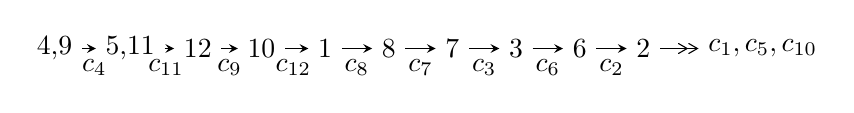
\begin{tikzpicture}[x=23pt, y=7pt]
	% node
	\node (A0) at (-1/8, 0) {4,9};
	\node (A1) at (17/16, 0) {5,11};
	\node (A2) at (17/8, 0) {12};
	\node (A3) at (25/8, 0) {10};
	\node (A4) at (33/8, 0) {1};
	\node (A5) at (41/8, 0) {8};
	\node (A6) at (49/8, 0) {7};
	\node (A7) at (57/8, 0) {3};
	\node (A8) at (65/8, 0) {6};
	\node (A9) at (73/8, 0) {2};
	\node (C1) at (1/2, -1) {$c_{4}$};
	\node (C2) at (13/8, -1) {$c_{11}$};
	\node (C3) at (21/8, -1) {$c_{9}$};
	\node (C4) at (29/8, -1) {$c_{12}$};
	\node (C5) at (37/8, -1) {$c_{8}$};
	\node (C6) at (45/8, -1) {$c_{7}$};
	\node (C7) at (53/8, -1) {$c_{3}$};
	\node (C8) at (61/8, -1) {$c_{6}$};
	\node (C9) at (69/8, -1) {$c_{2}$};
	\node (A10) at (11, 0) {$c_{1},c_{5},c_{10}$};

	% edge
	\draw[->,>=stealth]	
	(A0) edge (A1) (A1) edge (A2) (A2) edge (A3) (A3) edge (A4) (A4) edge (A5) (A5) edge (A6) (A6) edge (A7) (A7) edge (A8) (A8) edge (A9) ;
	\draw[->>,>={angle 60}]	
	(A9) edge (A10);
\end{tikzpicture} \\ 

\end{tabular} \\

\footnotetext{
The image of knot diagram is generated by the software ``\textbf{Draw programme}" developed by Andrew Bartholomew(\url{http://www.layer8.co.uk/maths/draw/index.htm\#Running-draw}), where we modified some parts for our purpose(\url{https://github.com/CATsTAILs/LinksPainter}).
}\phantom \\ \newline 
\centering \textbf{Ideals for irreducible components\footnotemark of $X_{\text{par}}$} 
 
\begin{align*}
I^u_{1}&=\langle 
-3.88782\times10^{23} u^{13}-5.12763\times10^{24} u^{12}+\cdots+2.64685\times10^{25} b+6.25813\times10^{25},\\
\phantom{I^u_{1}}&\phantom{= \langle  }7.50387\times10^{22} u^{13}+1.45176\times10^{23} u^{12}+\cdots+5.29369\times10^{25} a+2.07299\times10^{26},\\
\phantom{I^u_{1}}&\phantom{= \langle  }u^{14}+13 u^{13}+\cdots-32 u+64\rangle \\
I^u_{2}&=\langle 
u^7+u^6-3 u^5-2 u^4+3 u^3+b+2,\;u^7+u^6-3 u^5-2 u^4+3 u^3+a+2,\;u^8+u^7-3 u^6-2 u^5+3 u^4+2 u-1\rangle \\
\\
I^v_{1}&=\langle 
a,\;251 v^5+1517 v^4+2839 v^3+6155 v^2+413 b+3834 v+768,\;v^6+6 v^5+11 v^4+24 v^3+15 v^2+3 v+1\rangle \\
\end{align*}
\raggedright * 3 irreducible components of $\dim_{\mathbb{C}}=0$, with total 28 representations.\\
\footnotetext{All coefficients of polynomials are rational numbers. But the coefficients are sometimes approximated in decimal forms when there is not enough margin.}
\newpage
\renewcommand{\arraystretch}{1}
\centering \section*{I. $I^u_{1}= \langle -3.89\times10^{23} u^{13}-5.13\times10^{24} u^{12}+\cdots+2.65\times10^{25} b+6.26\times10^{25},\;7.50\times10^{22} u^{13}+1.45\times10^{23} u^{12}+\cdots+5.29\times10^{25} a+2.07\times10^{26},\;u^{14}+13 u^{13}+\cdots-32 u+64 \rangle$}
\flushleft \textbf{(i) Arc colorings}\\
\begin{tabular}{m{7pt} m{180pt} m{7pt} m{180pt} }
\flushright $a_{4}=$&$\begin{pmatrix}1\\0\end{pmatrix}$ \\
\flushright $a_{9}=$&$\begin{pmatrix}0\\u\end{pmatrix}$ \\
\flushright $a_{5}=$&$\begin{pmatrix}1\\u^2\end{pmatrix}$ \\
\flushright $a_{11}=$&$\begin{pmatrix}-0.00141751 u^{13}-0.00274243 u^{12}+\cdots-2.48245 u-3.91596\\0.0146885 u^{13}+0.193726 u^{12}+\cdots-5.56422 u-2.36437\end{pmatrix}$ \\
\flushright $a_{12}=$&$\begin{pmatrix}-0.00141751 u^{13}-0.00274243 u^{12}+\cdots-2.48245 u-3.91596\\0.0101820 u^{13}+0.140392 u^{12}+\cdots-4.97157 u-3.36822\end{pmatrix}$ \\
\flushright $a_{10}=$&$\begin{pmatrix}-0.00113062 u^{13}-0.0125080 u^{12}+\cdots-2.90912 u-1.42506\\0.0142858 u^{13}+0.186357 u^{12}+\cdots-5.61762 u-1.88242\end{pmatrix}$ \\
\flushright $a_{1}=$&$\begin{pmatrix}-0.0210436 u^{13}-0.266521 u^{12}+\cdots+3.80828 u-0.914411\\-0.0113459 u^{13}-0.139334 u^{12}+\cdots+2.52961 u-1.68257\end{pmatrix}$ \\
\flushright $a_{8}=$&$\begin{pmatrix}u\\u\end{pmatrix}$ \\
\flushright $a_{7}=$&$\begin{pmatrix}0.0181604 u^{13}+0.234062 u^{12}+\cdots-2.85095 u-0.317190\\-0.00288324 u^{13}-0.0324588 u^{12}+\cdots+0.957338 u-1.23160\end{pmatrix}$ \\
\flushright $a_{3}=$&$\begin{pmatrix}-0.00413905 u^{13}-0.0558999 u^{12}+\cdots+0.679785 u+1.52829\\-0.00466437 u^{13}-0.0566994 u^{12}+\cdots+0.968533 u-0.525572\end{pmatrix}$ \\
\flushright $a_{6}=$&$\begin{pmatrix}0.00922038 u^{13}+0.124297 u^{12}+\cdots-0.666608 u-1.67826\\-0.00752145 u^{13}-0.0902797 u^{12}+\cdots+1.73607 u-1.64474\end{pmatrix}$ \\
\flushright $a_{2}=$&$\begin{pmatrix}-0.0194805 u^{13}-0.252321 u^{12}+\cdots+2.53552 u+0.574034\\-0.0151718 u^{13}-0.187049 u^{12}+\cdots+2.63035 u-1.84661\end{pmatrix}$\\&\end{tabular}
\flushleft \textbf{(ii) Obstruction class $= -1$}\\~\\
\flushleft \textbf{(iii) Cusp Shapes $= \frac{6397031736972176627304075}{26468471689247551065891424} u^{13}+\frac{85735105186510577411506669}{26468471689247551065891424} u^{12}+\cdots-\frac{114004214719555496517015677}{827139740288985970809107} u-\frac{55506637637800758601432107}{827139740288985970809107}$}\\~\\
\newpage\renewcommand{\arraystretch}{1}
\flushleft \textbf{(iv) u-Polynomials at the component}\newline \\
\begin{tabular}{m{50pt}|m{274pt}}
Crossings & \hspace{64pt}u-Polynomials at each crossing \\
\hline $$\begin{aligned}c_{1},c_{6}\end{aligned}$$&$\begin{aligned}
&u^{14}+9 u^{13}+\cdots+16 u+1
\end{aligned}$\\
\hline $$\begin{aligned}c_{2},c_{5}\end{aligned}$$&$\begin{aligned}
&u^{14}+3 u^{13}+\cdots+8 u+1
\end{aligned}$\\
\hline $$\begin{aligned}c_{3}\end{aligned}$$&$\begin{aligned}
&u^{14}-61 u^{13}+\cdots+58652 u+7489
\end{aligned}$\\
\hline $$\begin{aligned}c_{4},c_{8}\end{aligned}$$&$\begin{aligned}
&u^{14}+13 u^{13}+\cdots-32 u+64
\end{aligned}$\\
\hline $$\begin{aligned}c_{7},c_{10}\end{aligned}$$&$\begin{aligned}
&u^{14}+41 u^{13}+\cdots-640 u+256
\end{aligned}$\\
\hline $$\begin{aligned}c_{9},c_{11},c_{12}\end{aligned}$$&$\begin{aligned}
&u^{14}-21 u^{13}+\cdots+17 u+1
\end{aligned}$\\
\hline
\end{tabular}\\~\\
\newpage\renewcommand{\arraystretch}{1}
\flushleft \textbf{(v) Riley Polynomials at the component}\newline \\
\begin{tabular}{m{50pt}|m{274pt}}
Crossings & \hspace{64pt}Riley Polynomials at each crossing \\
\hline $$\begin{aligned}c_{1},c_{6}\end{aligned}$$&$\begin{aligned}
&y^{14}-13 y^{13}+\cdots-32 y+1
\end{aligned}$\\
\hline $$\begin{aligned}c_{2},c_{5}\end{aligned}$$&$\begin{aligned}
&y^{14}-9 y^{13}+\cdots-16 y+1
\end{aligned}$\\
\hline $$\begin{aligned}c_{3}\end{aligned}$$&$\begin{aligned}
&y^{14}-3381 y^{13}+\cdots-1276544916 y+56085121
\end{aligned}$\\
\hline $$\begin{aligned}c_{4},c_{8}\end{aligned}$$&$\begin{aligned}
&y^{14}-339 y^{13}+\cdots-62464 y+4096
\end{aligned}$\\
\hline $$\begin{aligned}c_{7},c_{10}\end{aligned}$$&$\begin{aligned}
&y^{14}-1029 y^{13}+\cdots-2539520 y+65536
\end{aligned}$\\
\hline $$\begin{aligned}c_{9},c_{11},c_{12}\end{aligned}$$&$\begin{aligned}
&y^{14}-121 y^{13}+\cdots-57 y+1
\end{aligned}$\\
\hline
\end{tabular}\\~\\
\newpage\flushleft \textbf{(vi) Complex Volumes and Cusp Shapes}
$$\begin{array}{c|c|c}  
\text{Solutions to }I^u_{1}& \I (\text{vol} + \sqrt{-1}CS) & \text{Cusp shape}\\
 \hline 
\begin{aligned}
u &= -0.615322 + 0.027933 I \\
a &= \phantom{-}0.270955 + 0.334290 I \\
b &= -0.491780 - 0.018263 I\end{aligned}
 & -0.755939 - 0.001558 I & -11.59104 + 0.05980 I \\ \hline\begin{aligned}
u &= -0.615322 - 0.027933 I \\
a &= \phantom{-}0.270955 - 0.334290 I \\
b &= -0.491780 + 0.018263 I\end{aligned}
 & -0.755939 + 0.001558 I & -11.59104 - 0.05980 I \\ \hline\begin{aligned}
u &= \phantom{-}0.009870 + 0.545956 I \\
a &= -0.167508 + 0.354571 I \\
b &= -0.343156 + 1.170610 I\end{aligned}
 & \phantom{-}2.39955 + 2.72347 I & -2.27719 - 1.42875 I \\ \hline\begin{aligned}
u &= \phantom{-}0.009870 - 0.545956 I \\
a &= -0.167508 - 0.354571 I \\
b &= -0.343156 - 1.170610 I\end{aligned}
 & \phantom{-}2.39955 - 2.72347 I & -2.27719 + 1.42875 I \\ \hline\begin{aligned}
u &= \phantom{-}0.538862\phantom{ +0.000000I} \\
a &= \phantom{-}2.91010\phantom{ +0.000000I} \\
b &= \phantom{-}0.103022\phantom{ +0.000000I}\end{aligned}
 & -10.2297\phantom{ +0.000000I} & -34.5740\phantom{ +0.000000I} \\ \hline\begin{aligned}
u &= -0.527756\phantom{ +0.000000I} \\
a &= \phantom{-}0.348493\phantom{ +0.000000I} \\
b &= -0.450251\phantom{ +0.000000I}\end{aligned}
 & -0.765092\phantom{ +0.000000I} & -12.2670\phantom{ +0.000000I} \\ \hline\begin{aligned}
u &= \phantom{-}0.328130\phantom{ +0.000000I} \\
a &= -2.96230\phantom{ +0.000000I} \\
b &= -3.66807\phantom{ +0.000000I}\end{aligned}
 & -2.58775\phantom{ +0.000000I} & -102.750\phantom{ +0.000000I} \\ \hline\begin{aligned}
u &= \phantom{-}2.36859 + 0.76389 I \\
a &= \phantom{-}0.286166 - 0.684183 I \\
b &= \phantom{-}0.464252 + 0.349923 I\end{aligned}
 & -3.81801 - 4.65772 I & -14.3487 + 2.2929 I \\ \hline\begin{aligned}
u &= \phantom{-}2.36859 - 0.76389 I \\
a &= \phantom{-}0.286166 + 0.684183 I \\
b &= \phantom{-}0.464252 - 0.349923 I\end{aligned}
 & -3.81801 + 4.65772 I & -14.3487 - 2.2929 I \\ \hline\begin{aligned}
u &= -1.88270 + 1.66535 I \\
a &= -0.845008 - 0.271270 I \\
b &= -2.08577 - 0.29493 I\end{aligned}
 & \phantom{-}15.9880 + 11.7884 I & -14.3165 - 4.7631 I\\
 \hline 
 \end{array}$$\newpage$$\begin{array}{c|c|c}  
\text{Solutions to }I^u_{1}& \I (\text{vol} + \sqrt{-1}CS) & \text{Cusp shape}\\
 \hline 
\begin{aligned}
u &= -1.88270 - 1.66535 I \\
a &= -0.845008 + 0.271270 I \\
b &= -2.08577 + 0.29493 I\end{aligned}
 & \phantom{-}15.9880 - 11.7884 I & -14.3165 + 4.7631 I \\ \hline\begin{aligned}
u &= \phantom{-}2.40458 + 1.69377 I \\
a &= \phantom{-}0.839800 - 0.202162 I \\
b &= \phantom{-}2.14114 - 0.18650 I\end{aligned}
 & \phantom{-}17.5291 - 4.7891 I & -13.20379 + 0.61326 I \\ \hline\begin{aligned}
u &= \phantom{-}2.40458 - 1.69377 I \\
a &= \phantom{-}0.839800 + 0.202162 I \\
b &= \phantom{-}2.14114 + 0.18650 I\end{aligned}
 & \phantom{-}17.5291 + 4.7891 I & -13.20379 - 0.61326 I \\ \hline\begin{aligned}
u &= -17.9093\phantom{ +0.000000I} \\
a &= -0.565105\phantom{ +0.000000I} \\
b &= -2.35407\phantom{ +0.000000I}\end{aligned}
 & \phantom{-}6.82503\phantom{ +0.000000I} & \phantom{-0.000000 } 0\\
 \hline 
 \end{array}$$\newpage\newpage\renewcommand{\arraystretch}{1}
\centering \section*{II. $I^u_{2}= \langle u^7+u^6-3 u^5-2 u^4+3 u^3+b+2,\;u^7+u^6-3 u^5-2 u^4+3 u^3+a+2,\;u^8+u^7-3 u^6-2 u^5+3 u^4+2 u-1 \rangle$}
\flushleft \textbf{(i) Arc colorings}\\
\begin{tabular}{m{7pt} m{180pt} m{7pt} m{180pt} }
\flushright $a_{4}=$&$\begin{pmatrix}1\\0\end{pmatrix}$ \\
\flushright $a_{9}=$&$\begin{pmatrix}0\\u\end{pmatrix}$ \\
\flushright $a_{5}=$&$\begin{pmatrix}1\\u^2\end{pmatrix}$ \\
\flushright $a_{11}=$&$\begin{pmatrix}- u^7- u^6+3 u^5+2 u^4-3 u^3-2\\- u^7- u^6+3 u^5+2 u^4-3 u^3-2\end{pmatrix}$ \\
\flushright $a_{12}=$&$\begin{pmatrix}- u^7- u^6+3 u^5+2 u^4-3 u^3-2\\- u^7- u^6+3 u^5+2 u^4-3 u^3- u-2\end{pmatrix}$ \\
\flushright $a_{10}=$&$\begin{pmatrix}- u^7- u^6+3 u^5+2 u^4-3 u^3-2\\- u^7- u^6+3 u^5+2 u^4-3 u^3-2\end{pmatrix}$ \\
\flushright $a_{1}=$&$\begin{pmatrix}0\\- u\end{pmatrix}$ \\
\flushright $a_{8}=$&$\begin{pmatrix}u\\u\end{pmatrix}$ \\
\flushright $a_{7}=$&$\begin{pmatrix}u\\u\end{pmatrix}$ \\
\flushright $a_{3}=$&$\begin{pmatrix}- u^2+1\\- u^2\end{pmatrix}$ \\
\flushright $a_{6}=$&$\begin{pmatrix}- u^3+2 u\\- u^5+u^3+u\end{pmatrix}$ \\
\flushright $a_{2}=$&$\begin{pmatrix}u^5-2 u^3+u\\u^5- u^3- u\end{pmatrix}$\\&\end{tabular}
\flushleft \textbf{(ii) Obstruction class $= 1$}\\~\\
\flushleft \textbf{(iii) Cusp Shapes $= 8 u^7+8 u^6-18 u^5-12 u^4+7 u^3-3 u^2+12 u-3$}\\~\\
\newpage\renewcommand{\arraystretch}{1}
\flushleft \textbf{(iv) u-Polynomials at the component}\newline \\
\begin{tabular}{m{50pt}|m{274pt}}
Crossings & \hspace{64pt}u-Polynomials at each crossing \\
\hline $$\begin{aligned}c_{1}\end{aligned}$$&$\begin{aligned}
&u^8-3 u^7+7 u^6-10 u^5+11 u^4-10 u^3+6 u^2-4 u+1
\end{aligned}$\\
\hline $$\begin{aligned}c_{2}\end{aligned}$$&$\begin{aligned}
&u^8- u^7- u^6+2 u^5+u^4-2 u^3+2 u-1
\end{aligned}$\\
\hline $$\begin{aligned}c_{3},c_{4}\end{aligned}$$&$\begin{aligned}
&u^8+u^7-3 u^6-2 u^5+3 u^4+2 u-1
\end{aligned}$\\
\hline $$\begin{aligned}c_{5}\end{aligned}$$&$\begin{aligned}
&u^8+u^7- u^6-2 u^5+u^4+2 u^3-2 u-1
\end{aligned}$\\
\hline $$\begin{aligned}c_{6}\end{aligned}$$&$\begin{aligned}
&u^8+3 u^7+7 u^6+10 u^5+11 u^4+10 u^3+6 u^2+4 u+1
\end{aligned}$\\
\hline $$\begin{aligned}c_{7},c_{10}\end{aligned}$$&$\begin{aligned}
&u^8
\end{aligned}$\\
\hline $$\begin{aligned}c_{8}\end{aligned}$$&$\begin{aligned}
&u^8- u^7-3 u^6+2 u^5+3 u^4-2 u-1
\end{aligned}$\\
\hline $$\begin{aligned}c_{9}\end{aligned}$$&$\begin{aligned}
&(u-1)^8
\end{aligned}$\\
\hline $$\begin{aligned}c_{11},c_{12}\end{aligned}$$&$\begin{aligned}
&(u+1)^8
\end{aligned}$\\
\hline
\end{tabular}\\~\\
\newpage\renewcommand{\arraystretch}{1}
\flushleft \textbf{(v) Riley Polynomials at the component}\newline \\
\begin{tabular}{m{50pt}|m{274pt}}
Crossings & \hspace{64pt}Riley Polynomials at each crossing \\
\hline $$\begin{aligned}c_{1},c_{6}\end{aligned}$$&$\begin{aligned}
&y^8+5 y^7+11 y^6+6 y^5-17 y^4-34 y^3-22 y^2-4 y+1
\end{aligned}$\\
\hline $$\begin{aligned}c_{2},c_{5}\end{aligned}$$&$\begin{aligned}
&y^8-3 y^7+7 y^6-10 y^5+11 y^4-10 y^3+6 y^2-4 y+1
\end{aligned}$\\
\hline $$\begin{aligned}c_{3},c_{4},c_{8}\end{aligned}$$&$\begin{aligned}
&y^8-7 y^7+19 y^6-22 y^5+3 y^4+14 y^3-6 y^2-4 y+1
\end{aligned}$\\
\hline $$\begin{aligned}c_{7},c_{10}\end{aligned}$$&$\begin{aligned}
&y^8
\end{aligned}$\\
\hline $$\begin{aligned}c_{9},c_{11},c_{12}\end{aligned}$$&$\begin{aligned}
&(y-1)^8
\end{aligned}$\\
\hline
\end{tabular}\\~\\
\newpage\flushleft \textbf{(vi) Complex Volumes and Cusp Shapes}
$$\begin{array}{c|c|c}  
\text{Solutions to }I^u_{2}& \I (\text{vol} + \sqrt{-1}CS) & \text{Cusp shape}\\
 \hline 
\begin{aligned}
u &= \phantom{-}1.180120 + 0.268597 I \\
a &= -0.805639 + 0.183365 I \\
b &= -0.805639 + 0.183365 I\end{aligned}
 & -2.68559 - 1.13123 I & -13.78185 + 1.82144 I \\ \hline\begin{aligned}
u &= \phantom{-}1.180120 - 0.268597 I \\
a &= -0.805639 - 0.183365 I \\
b &= -0.805639 - 0.183365 I\end{aligned}
 & -2.68559 + 1.13123 I & -13.78185 - 1.82144 I \\ \hline\begin{aligned}
u &= \phantom{-}0.108090 + 0.747508 I \\
a &= -0.189481 + 1.310380 I \\
b &= -0.189481 + 1.310380 I\end{aligned}
 & \phantom{-}0.51448 - 2.57849 I & -9.42408 + 5.06085 I \\ \hline\begin{aligned}
u &= \phantom{-}0.108090 - 0.747508 I \\
a &= -0.189481 - 1.310380 I \\
b &= -0.189481 - 1.310380 I\end{aligned}
 & \phantom{-}0.51448 + 2.57849 I & -9.42408 - 5.06085 I \\ \hline\begin{aligned}
u &= -1.37100\phantom{ +0.000000I} \\
a &= \phantom{-}0.729394\phantom{ +0.000000I} \\
b &= \phantom{-}0.729394\phantom{ +0.000000I}\end{aligned}
 & -8.14766\phantom{ +0.000000I} & -18.0480\phantom{ +0.000000I} \\ \hline\begin{aligned}
u &= -1.334530 + 0.318930 I \\
a &= \phantom{-}0.708845 + 0.169402 I \\
b &= \phantom{-}0.708845 + 0.169402 I\end{aligned}
 & -4.02461 + 6.44354 I & -15.1664 - 7.9255 I \\ \hline\begin{aligned}
u &= -1.334530 - 0.318930 I \\
a &= \phantom{-}0.708845 - 0.169402 I \\
b &= \phantom{-}0.708845 - 0.169402 I\end{aligned}
 & -4.02461 - 6.44354 I & -15.1664 + 7.9255 I \\ \hline\begin{aligned}
u &= \phantom{-}0.463640\phantom{ +0.000000I} \\
a &= -2.15684\phantom{ +0.000000I} \\
b &= -2.15684\phantom{ +0.000000I}\end{aligned}
 & -2.48997\phantom{ +0.000000I} & \phantom{-}1.79260\phantom{ +0.000000I}\\
 \hline 
 \end{array}$$\newpage\newpage\renewcommand{\arraystretch}{1}
\centering \section*{III. $I^v_{1}= \langle a,\;251 v^5+1517 v^4+\cdots+413 b+768,\;v^6+6 v^5+11 v^4+24 v^3+15 v^2+3 v+1 \rangle$}
\flushleft \textbf{(i) Arc colorings}\\
\begin{tabular}{m{7pt} m{180pt} m{7pt} m{180pt} }
\flushright $a_{4}=$&$\begin{pmatrix}1\\0\end{pmatrix}$ \\
\flushright $a_{9}=$&$\begin{pmatrix}v\\0\end{pmatrix}$ \\
\flushright $a_{5}=$&$\begin{pmatrix}1\\0\end{pmatrix}$ \\
\flushright $a_{11}=$&$\begin{pmatrix}0\\-0.607748 v^{5}-3.67312 v^{4}+\cdots-9.28329 v-1.85956\end{pmatrix}$ \\
\flushright $a_{12}=$&$\begin{pmatrix}0.0290557 v^{5}+0.0242131 v^{4}+\cdots-0.687651 v-0.0266344\\-0.607748 v^{5}-3.67312 v^{4}+\cdots-9.28329 v-1.85956\end{pmatrix}$ \\
\flushright $a_{10}=$&$\begin{pmatrix}-0.0290557 v^{5}-0.0242131 v^{4}+\cdots+0.687651 v+0.0266344\\-0.392252 v^{5}-2.32688 v^{4}+\cdots-5.71671 v-1.14044\end{pmatrix}$ \\
\flushright $a_{1}=$&$\begin{pmatrix}- v\\-0.392252 v^{5}-2.32688 v^{4}+\cdots-5.71671 v-1.14044\end{pmatrix}$ \\
\flushright $a_{8}=$&$\begin{pmatrix}v\\0\end{pmatrix}$ \\
\flushright $a_{7}=$&$\begin{pmatrix}v\\0.392252 v^{5}+2.32688 v^{4}+\cdots+5.71671 v+1.14044\end{pmatrix}$ \\
\flushright $a_{3}=$&$\begin{pmatrix}0.0266344 v^{5}+0.188862 v^{4}+\cdots+0.0363196 v+1.39225\\-0.421308 v^{5}-2.35109 v^{4}+\cdots-3.02906 v+0.886199\end{pmatrix}$ \\
\flushright $a_{6}=$&$\begin{pmatrix}0.392252 v^{5}+2.32688 v^{4}+\cdots+6.71671 v+1.14044\\0.392252 v^{5}+2.32688 v^{4}+\cdots+5.71671 v+1.14044\end{pmatrix}$ \\
\flushright $a_{2}=$&$\begin{pmatrix}0.569007 v^{5}+3.30751 v^{4}+\cdots+6.86683 v+1.56174\\-0.0290557 v^{5}-0.0242131 v^{4}+\cdots+2.68765 v+1.02663\end{pmatrix}$\\&\end{tabular}
\flushleft \textbf{(ii) Obstruction class $= 1$}\\~\\
\flushleft \textbf{(iii) Cusp Shapes $= \frac{1191}{413} v^5+\frac{6981}{413} v^4+\frac{11931}{413} v^3+\frac{26206}{413} v^2+\frac{13113}{413} v-\frac{8216}{413}$}\\~\\
\newpage\renewcommand{\arraystretch}{1}
\flushleft \textbf{(iv) u-Polynomials at the component}\newline \\
\begin{tabular}{m{50pt}|m{274pt}}
Crossings & \hspace{64pt}u-Polynomials at each crossing \\
\hline $$\begin{aligned}c_{1},c_{3}\end{aligned}$$&$\begin{aligned}
&(u^3- u^2+2 u-1)^2
\end{aligned}$\\
\hline $$\begin{aligned}c_{2}\end{aligned}$$&$\begin{aligned}
&(u^3+u^2-1)^2
\end{aligned}$\\
\hline $$\begin{aligned}c_{4},c_{8}\end{aligned}$$&$\begin{aligned}
&u^6
\end{aligned}$\\
\hline $$\begin{aligned}c_{5}\end{aligned}$$&$\begin{aligned}
&(u^3- u^2+1)^2
\end{aligned}$\\
\hline $$\begin{aligned}c_{6}\end{aligned}$$&$\begin{aligned}
&(u^3+u^2+2 u+1)^2
\end{aligned}$\\
\hline $$\begin{aligned}c_{7},c_{9}\end{aligned}$$&$\begin{aligned}
&(u^2+u-1)^3
\end{aligned}$\\
\hline $$\begin{aligned}c_{10},c_{11},c_{12}\end{aligned}$$&$\begin{aligned}
&(u^2- u-1)^3
\end{aligned}$\\
\hline
\end{tabular}\\~\\
\newpage\renewcommand{\arraystretch}{1}
\flushleft \textbf{(v) Riley Polynomials at the component}\newline \\
\begin{tabular}{m{50pt}|m{274pt}}
Crossings & \hspace{64pt}Riley Polynomials at each crossing \\
\hline $$\begin{aligned}c_{1},c_{3},c_{6}\end{aligned}$$&$\begin{aligned}
&(y^3+3 y^2+2 y-1)^2
\end{aligned}$\\
\hline $$\begin{aligned}c_{2},c_{5}\end{aligned}$$&$\begin{aligned}
&(y^3- y^2+2 y-1)^2
\end{aligned}$\\
\hline $$\begin{aligned}c_{4},c_{8}\end{aligned}$$&$\begin{aligned}
&y^6
\end{aligned}$\\
\hline $$\begin{aligned}c_{7},c_{9},c_{10}\\c_{11},c_{12}\end{aligned}$$&$\begin{aligned}
&(y^2-3 y+1)^3
\end{aligned}$\\
\hline
\end{tabular}\\~\\
\newpage\flushleft \textbf{(vi) Complex Volumes and Cusp Shapes}
$$\begin{array}{c|c|c}  
\text{Solutions to }I^v_{1}& \I (\text{vol} + \sqrt{-1}CS) & \text{Cusp shape}\\
 \hline 
\begin{aligned}
v &= -0.670304\phantom{ +0.000000I} \\
a &= \phantom{-0.000000 } 0 \\
b &= -0.922021\phantom{ +0.000000I}\end{aligned}
 & -2.10041\phantom{ +0.000000I} & -18.3450\phantom{ +0.000000I} \\ \hline\begin{aligned}
v &= -0.046814 + 0.284512 I \\
a &= \phantom{-0.000000 } 0 \\
b &= -0.34801 - 2.11500 I\end{aligned}
 & \phantom{-}2.03717 - 2.82812 I & -25.9630 + 6.8067 I \\ \hline\begin{aligned}
v &= -0.046814 - 0.284512 I \\
a &= \phantom{-0.000000 } 0 \\
b &= -0.34801 + 2.11500 I\end{aligned}
 & \phantom{-}2.03717 + 2.82812 I & -25.9630 - 6.8067 I \\ \hline\begin{aligned}
v &= -0.32087 + 1.95007 I \\
a &= \phantom{-0.000000 } 0 \\
b &= \phantom{-}0.132927 + 0.807858 I\end{aligned}
 & -5.85852 - 2.82812 I & -18.4326 + 1.8100 I \\ \hline\begin{aligned}
v &= -0.32087 - 1.95007 I \\
a &= \phantom{-0.000000 } 0 \\
b &= \phantom{-}0.132927 - 0.807858 I\end{aligned}
 & -5.85852 + 2.82812 I & -18.4326 - 1.8100 I \\ \hline\begin{aligned}
v &= -4.59433\phantom{ +0.000000I} \\
a &= \phantom{-0.000000 } 0 \\
b &= \phantom{-}0.352181\phantom{ +0.000000I}\end{aligned}
 & -9.99610\phantom{ +0.000000I} & \phantom{-}0.135730\phantom{ +0.000000I}\\
 \hline 
 \end{array}$$\newpage
\newpage\renewcommand{\arraystretch}{1}
\centering \section*{ IV. u-Polynomials}
\begin{tabular}{m{50pt}|m{274pt}}
Crossings & \hspace{64pt}u-Polynomials at each crossing \\
\hline $$\begin{aligned}c_{1}\end{aligned}$$&$\begin{aligned}
&(u^3- u^2+2 u-1)^2\\
&\cdot(u^8-3 u^7+7 u^6-10 u^5+11 u^4-10 u^3+6 u^2-4 u+1)\\
&\cdot(u^{14}+9 u^{13}+\cdots+16 u+1)
\end{aligned}$\\
\hline $$\begin{aligned}c_{2}\end{aligned}$$&$\begin{aligned}
&(u^3+u^2-1)^2(u^8- u^7- u^6+2 u^5+u^4-2 u^3+2 u-1)\\
&\cdot(u^{14}+3 u^{13}+\cdots+8 u+1)
\end{aligned}$\\
\hline $$\begin{aligned}c_{3}\end{aligned}$$&$\begin{aligned}
&(u^3- u^2+2 u-1)^2(u^8+u^7-3 u^6-2 u^5+3 u^4+2 u-1)\\
&\cdot(u^{14}-61 u^{13}+\cdots+58652 u+7489)
\end{aligned}$\\
\hline $$\begin{aligned}c_{4}\end{aligned}$$&$\begin{aligned}
&u^6(u^8+u^7+\cdots+2 u-1)(u^{14}+13 u^{13}+\cdots-32 u+64)
\end{aligned}$\\
\hline $$\begin{aligned}c_{5}\end{aligned}$$&$\begin{aligned}
&(u^3- u^2+1)^2(u^8+u^7- u^6-2 u^5+u^4+2 u^3-2 u-1)\\
&\cdot(u^{14}+3 u^{13}+\cdots+8 u+1)
\end{aligned}$\\
\hline $$\begin{aligned}c_{6}\end{aligned}$$&$\begin{aligned}
&(u^3+u^2+2 u+1)^2\\
&\cdot(u^8+3 u^7+7 u^6+10 u^5+11 u^4+10 u^3+6 u^2+4 u+1)\\
&\cdot(u^{14}+9 u^{13}+\cdots+16 u+1)
\end{aligned}$\\
\hline $$\begin{aligned}c_{7}\end{aligned}$$&$\begin{aligned}
&u^8(u^2+u-1)^3(u^{14}+41 u^{13}+\cdots-640 u+256)
\end{aligned}$\\
\hline $$\begin{aligned}c_{8}\end{aligned}$$&$\begin{aligned}
&u^6(u^8- u^7+\cdots-2 u-1)(u^{14}+13 u^{13}+\cdots-32 u+64)
\end{aligned}$\\
\hline $$\begin{aligned}c_{9}\end{aligned}$$&$\begin{aligned}
&((u-1)^8)(u^2+u-1)^3(u^{14}-21 u^{13}+\cdots+17 u+1)
\end{aligned}$\\
\hline $$\begin{aligned}c_{10}\end{aligned}$$&$\begin{aligned}
&u^8(u^2- u-1)^3(u^{14}+41 u^{13}+\cdots-640 u+256)
\end{aligned}$\\
\hline $$\begin{aligned}c_{11},c_{12}\end{aligned}$$&$\begin{aligned}
&((u+1)^8)(u^2- u-1)^3(u^{14}-21 u^{13}+\cdots+17 u+1)
\end{aligned}$\\
\hline
\end{tabular}\newpage\renewcommand{\arraystretch}{1}
\centering \section*{ V. Riley Polynomials}
\begin{tabular}{m{50pt}|m{274pt}}
Crossings & \hspace{64pt}Riley Polynomials at each crossing \\
\hline $$\begin{aligned}c_{1},c_{6}\end{aligned}$$&$\begin{aligned}
&(y^3+3 y^2+2 y-1)^2\\
&\cdot(y^8+5 y^7+11 y^6+6 y^5-17 y^4-34 y^3-22 y^2-4 y+1)\\
&\cdot(y^{14}-13 y^{13}+\cdots-32 y+1)
\end{aligned}$\\
\hline $$\begin{aligned}c_{2},c_{5}\end{aligned}$$&$\begin{aligned}
&(y^3- y^2+2 y-1)^2\\
&\cdot(y^8-3 y^7+7 y^6-10 y^5+11 y^4-10 y^3+6 y^2-4 y+1)\\
&\cdot(y^{14}-9 y^{13}+\cdots-16 y+1)
\end{aligned}$\\
\hline $$\begin{aligned}c_{3}\end{aligned}$$&$\begin{aligned}
&(y^3+3 y^2+2 y-1)^2\\
&\cdot(y^8-7 y^7+19 y^6-22 y^5+3 y^4+14 y^3-6 y^2-4 y+1)\\
&\cdot(y^{14}-3381 y^{13}+\cdots-1276544916 y+56085121)
\end{aligned}$\\
\hline $$\begin{aligned}c_{4},c_{8}\end{aligned}$$&$\begin{aligned}
&y^6(y^8-7 y^7+19 y^6-22 y^5+3 y^4+14 y^3-6 y^2-4 y+1)\\
&\cdot(y^{14}-339 y^{13}+\cdots-62464 y+4096)
\end{aligned}$\\
\hline $$\begin{aligned}c_{7},c_{10}\end{aligned}$$&$\begin{aligned}
&y^8(y^2-3 y+1)^3(y^{14}-1029 y^{13}+\cdots-2539520 y+65536)
\end{aligned}$\\
\hline $$\begin{aligned}c_{9},c_{11},c_{12}\end{aligned}$$&$\begin{aligned}
&((y-1)^8)(y^2-3 y+1)^3(y^{14}-121 y^{13}+\cdots-57 y+1)
\end{aligned}$\\
\hline
\end{tabular}
\vskip 2pc
\end{document}